\section{Goals of the application}
From the analysis of client's needs for the software to be we can derive the following list of goals.
\subsection{Goals Passenger side}
A Passenger:
\begin{enumerate}
\item must be able to register to the service
\item must be able to login to the service
\item can choose to use both the web application and the mobile application
\item  must be able to choose between requesting an immediate taxi service or reserving one for the future
\item must receive, if a taxi is available for a immediate request, a notification stating the arrival time and the taxi identification number
\item if he has reserved a taxi correctly for a certain meeting time, must be notified before that time with a notification saying the arrival time of the taxi and it identification number, or, in case of problems, saying the nature of the problem.
\end{enumerate}
\subsection{Goals Taxi Driver side}
A Taxi Driver:
\begin{enumerate}
\item must be able to set himself as available (start working) or not available (stop working)
\item must receive requests (both immediate and reservations) only if he is available 
\item must receive a notification, if he is the first taxi in the queue corresponding to his actual location and if a passenger made an immediate request in that zone
\item when available, must be set in the correct waiting queue
\item must receive the location of the passenger who made the request, if he accepted it
\end{enumerate}

\section{Derived behavior of the actors}
From the domain analysis, the assumptions and the basic requirements for the application we can derive a model of behavior of the agents (Passengers and Taxi Drivers) when they use the future application
\subsection{Passenger behavior}
\begin{figure}[H]
\centering
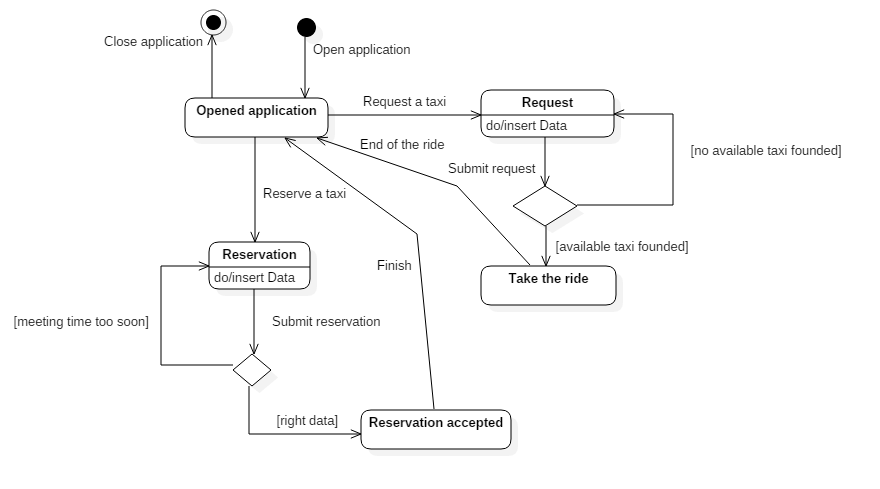
\includegraphics[scale=0.5]{Images/statechart_passenger}
\end{figure}
\subsection{Taxi Driver behavior}
\begin{figure}[H]
\centering
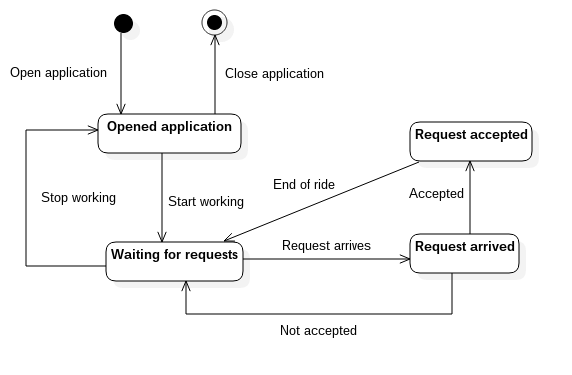
\includegraphics[scale=0.5]{Images/statechart_taxiDriver}
\end{figure}